\documentclass[tikz]{standalone}

\usepackage{pgfplots}
\pgfplotsset{compat=newest}

\usepackage{tkz-tab}
\usepackage{nicematrix}
\usetikzlibrary{angles,quotes,matrix,shapes.geometric}

\begin{document}

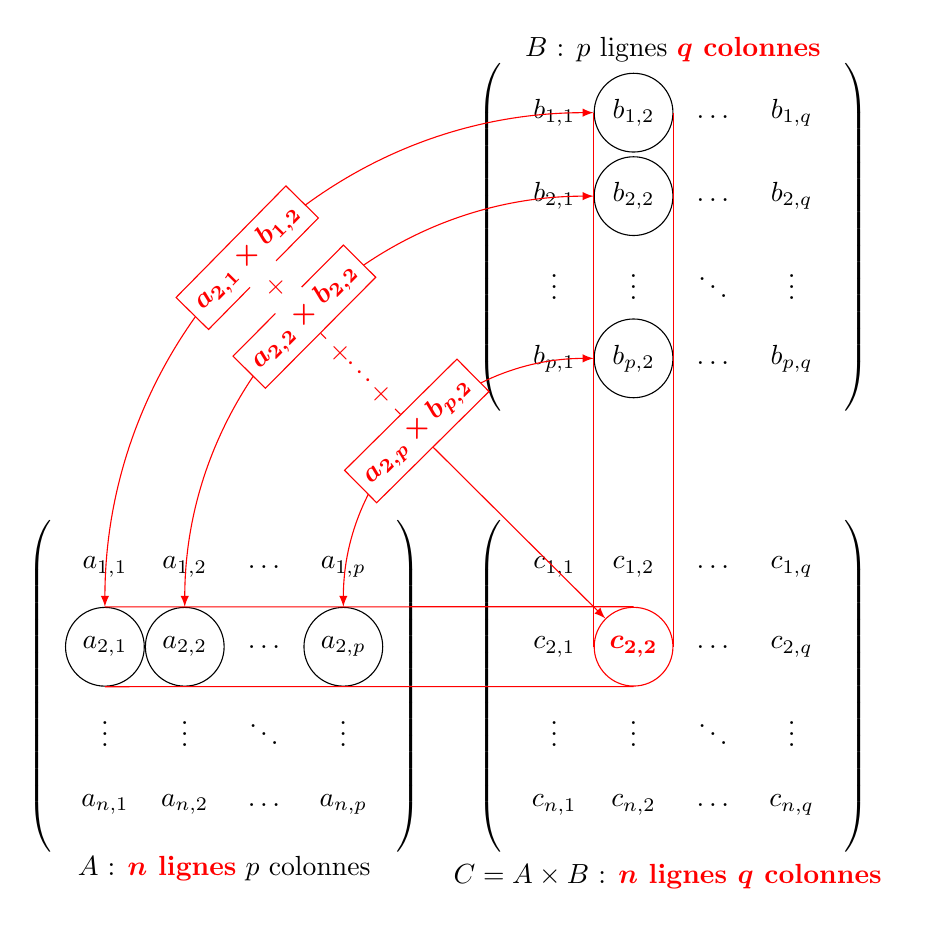
\begin{tikzpicture}[scale=0.95, >=latex,
	node style sp/.style={draw,circle,minimum size=1cm},
	node style ge/.style={circle,minimum size=1cm},
	arrow style mul/.style={draw,sloped,midway,fill=white},
	arrow style plus/.style={midway,sloped,fill=white}]
	% Matrice A
	\matrix (A) [matrix of math nodes,nodes={node style ge},left delimiter=(,right delimiter=)] at (0,0) {
		a_{1,1} & a_{1,2} & \ldots & a_{1,p} \\
		|[node style sp]| a_{2,1} & |[node style sp]| a_{2,2} & \ldots & |[node style sp]| a_{2,p} \\
		\vdots & \vdots & \ddots & \vdots \\
		a_{n,1} & a_{n,2} & \ldots & a_{n,p} \\ };
	\node[below=-3pt] at (A.south) {$A$ : \textcolor{red}{\bfseries\boldmath $n$ \unboldmath lignes} $p$ colonnes};
	% Matrice B
	\matrix (B) [matrix of math nodes,nodes={node style ge},left delimiter=(,right delimiter=)] at (6cm,6cm) {
		b_{1,1} & |[node style sp]| b_{1,2} & \ldots & b_{1,q} \\
		b_{2,1} & |[node style sp]| b_{2,2} & \ldots & b_{2,q} \\
		\vdots & \vdots & \ddots & \vdots \\
		b_{p,1} & |[node style sp]| b_{p,2} & \ldots & b_{p,q} \\ };
	\node[above=-3pt] at (B.north) {$B$ : $p$ lignes \textcolor{red}{\bfseries\boldmath $q$ \unboldmath colonnes}};
	% Matrice résultat C
	\matrix (C) [matrix of math nodes,nodes={node style ge},left delimiter=(,right delimiter=)] at (6cm,0) {
		c_{1,1} & c_{1,2} & \ldots & c_{1,q} \\
		c_{2,1} & |[node style sp,red]| \text{\boldmath$c_{2,2}$} & \ldots & c_{2,q} \\
		\vdots & \vdots & \ddots & \vdots \\
		c_{n,1} & c_{n,2} & \ldots & c_{n,q} \\ };
	\node [below=0pt] at (C.south) {$C=A\times B$ : \textcolor{red}{\bfseries\boldmath $n$ lignes $q$ colonnes \unboldmath}};
	% Les fleches
	\draw[red] (A-2-1.north) -- (C-2-2.north);
	\draw[red] (A-2-1.south) -- (C-2-2.south);
	\draw[red] (B-1-2.west) -- (C-2-2.west);
	\draw[red] (B-1-2.east) -- (C-2-2.east);
	\draw[<->,red] (A-2-1) to[in=180,out=90] node[arrow style mul] (x) {$\text{\boldmath $a_{2,1}\times b_{1,2}$}$} (B-1-2);
	\draw[<->,red] (A-2-2) to[in=180,out=90] node[arrow style mul] (y) {$\text{\boldmath $a_{2,2}\times b_{2,2}$}$} (B-2-2);
	\draw[<->,red] (A-2-4) to[in=180,out=90] node[arrow style mul] (z) {$\text{\boldmath $a_{2,p}\times b_{p,2}$}$} (B-4-2);
	\draw[->,red] (x) to node[arrow style plus] {$+$} (y) to node[arrow style plus] {$+\raisebox{.5ex}{\ldots}+$} (z) to (C-2-2.north west);
\end{tikzpicture}

\end{document}